\documentclass{article}
\usepackage[margin=1in]{geometry}
\usepackage{amsmath,amssymb}
\usepackage{booktabs}
\usepackage{multirow}
\usepackage{arydshln}
\usepackage{graphicx}
\usepackage{xcolor}
\usepackage{url}
\usepackage{hyperref}
\usepackage{microtype}
\usepackage{algorithm}
\usepackage{algpseudocode}
\usepackage{listings}
\usepackage[numbers]{natbib}
\usepackage{parskip}

\definecolor{fpgagreen}{RGB}{0,128,0}
\definecolor{paperred}{RGB}{200,0,0}

\title{\textbf{Don't Waste BRAM: FPGA-Aware KV Cache Quantization\\via Binary \{4,8\}-bit Bit-Width Selection}}

\author{
  Anonymous Submission\\
  \texttt{https://github.com/LonghornSilicon/dont-waste-bits}
}

\date{}

\begin{document}

\maketitle

\begin{abstract}
Dynamic KV cache quantization assigns variable bit-widths to attention keys and values during LLM inference. Prior work (DWB, arXiv:2604.04722) optimizes for \emph{average bits per token}, inadvertently including 2-bit quantization in the allocation despite its identical FPGA hardware cost to 4-bit on Xilinx Ultrascale+ BRAM. We show that the 2-bit option wastes no BRAM bandwidth while degrading accuracy from 41.6\% to 25.0\% on HellaSwag (SmolLM-360M). We propose an \emph{FPGA-aware binary \{4,8\}-bit} scheme trained with Gumbel-softmax that optimizes directly for FPGA BRAM cost rather than average bits. At SmolLM-360M (where INT4 is unconditionally lossless), the binary controller achieves 3.48$\times$ FPGA throughput over FP16---compared to DWB's 2.44$\times$ ($+$43\%)---at equal accuracy (41.0\% vs. 41.2\%), using 21\% fewer bits. At SmolLM-1.7B (where INT4 is lossy), the $\{4,8\}$-bit scheme produces a \emph{continuous} accuracy--speedup Pareto frontier. Our Pareto-best point is 5-seed validated at $n{=}500$ HellaSwag: $p_4{=}0.96$ achieves \textbf{47.72\%$\pm$1.03\,pp at 3.36$\times$ FPGA speedup --- $\mathbf{+38\%}$ throughput vs.\ DWB} (48.6\% @ 2.44$\times$) at within-seed-noise accuracy. Two additional 5-seed points anchor the frontier: $p_4{=}0.74$ (48.04\%$\pm$0.75\,pp, 2.80$\times$, $+$15\%) and $p_4{=}0.81$ (48.32\%$\pm$0.94\,pp, 2.96$\times$, $+$21\%). A controlled routing ablation (random vs.\ learned Gumbel vs.\ KV-norm vs.\ KV-norm \emph{inverted}) at the 74/26 split places all strategies within $\pm$1 seed-std, and the two KV-norm directions return \emph{identical} 44.5\% --- KV L2 norm is not a directional routing signal. At the right bit-set and ratio, per-token \emph{routing choice} carries no measurable accuracy signal above seed noise. We further establish a \emph{scale-dependent losslessness threshold}: effective quantization residual below 8.1\% (SmolLM-360M) is lossless INT4; above 12.4\% (SmolLM-1.7B) requires selective 8-bit upgrades. We introduce \emph{per-token quality proxies}---computed from actual quantization errors during signal extraction---that enable genuine mixed \{4,8\}-bit allocation at scales where global quality scores fail. We further derive a \emph{beta calibration criterion} ($\beta^* = \overline{q_{t,8} - q_{t,4}}/0.267$) that determines the optimal FPGA penalty weight from a $<$1 minute CPU calibration---validated across ten checkpoints and five model families (SmolLM/LLaMA-MHA, SmolLM2/LLaMA-GQA, TinyLlama/LLaMA-GQA, OPT/Meta, GPT/OpenAI; scales 124M--1.7B), with 9 of 10 within $\leq\pm0.04$. Key findings: GQA reduces gap\_mean vs.\ MHA at equal scale ($-$16\%) but floor convergence requires both GQA and $\geq$1B scale; a floor gap\_mean $\approx 0.18$--$0.19$ acts as a representation quality attractor reached by larger OPT models, GQA+scale, MHA instruction-tuning, and the complete GPT-2 family---validating that representation quality, not raw K/V dimension, is the dominant factor. Above the transition, a broad mixed-allocation plateau gives 2.52--2.93$\times$ speedup, all exceeding DWB. Our FPGA cost model, binary controller, and per-token quality method are released as a reference implementation at \url{https://github.com/LonghornSilicon/dont-waste-bits}.
\end{abstract}

\section{Introduction}

On-device LLMs face a memory bandwidth bottleneck: the KV cache grows linearly with sequence length and must be transferred from BRAM to compute units on every token generation step. Quantizing the KV cache to 4-bit precision reduces this bandwidth by 4$\times$ and can be nearly lossless for smaller models~\citep{liu2024kivi,hooper2024kvquant}.

Recent work (DWB;~\citep{haeri2026dwb}) proposes \emph{dynamic} bit-width allocation, assigning different bit-widths $b_t \in \{2, 4, 8, 16\}$ per token based on signal characteristics. DWB reports 17.75\% latency reduction over static 4-bit KV on Xilinx Ultrascale+ FPGA hardware. However, DWB's bit-width set includes 2-bit tokens, which comprise 47.9\% of DWB's allocation while providing no FPGA bandwidth saving over 4-bit.

\textbf{The core problem.} Xilinx Ultrascale+ BRAM has a minimum port width of 4 bits. Any quantization below 4 bits still occupies a 4-bit BRAM slot, providing no memory bandwidth reduction. Yet full 2-bit quantization reduces accuracy from 41.6\% to 25.0\% on HellaSwag (SmolLM-360M)---a catastrophic 16.6pp drop. DWB's controller selects the \emph{least important} tokens for 2-bit (lower attention weights), so their specific 2-bit tokens may be less harmful than full 2-bit. But the FPGA argument holds regardless of token selection: those same tokens could be stored at 4-bit precision with \emph{identical BRAM cost} and strictly better representational accuracy. There is no reason to choose 2-bit on this hardware.

Our contributions are:

\begin{enumerate}
\item \textbf{FPGA BRAM cost model}: A formal model of Xilinx Ultrascale+ BRAM port access costs showing that 2-bit quantization occupies the same 4-bit port slot as 4-bit---providing zero bandwidth savings---while catastrophically degrading accuracy ($-$16.6pp). This exposes a fundamental design flaw in DWB that causes it to spend 47.9\% of allocation on a strictly dominated option.

\item \textbf{Binary \{4,8\}-bit scheme}: By restricting bit choices to $\{4, 8\}$---the only two options with distinct BRAM costs---we simplify the allocation to a single binary decision per token. At SmolLM-360M (where INT4 is lossless), the learned controller correctly converges to 100\% 4-bit, achieving 3.48$\times$ FPGA speedup vs.\ DWB's 2.44$\times$ entirely by eliminating wasteful 2-bit tokens. At SmolLM-1.7B (where INT4 degrades $-$7.9pp), our Pareto-best 5-seed validated point is $p_4{=}0.96$: \textbf{47.72\%$\pm$1.03\,pp at 3.36$\times$ FPGA speedup (\mbox{$+$38\%} throughput vs.\ DWB)} --- within 1\,pp of DWB's 48.6\% and within seed-noise of our own $p_4{=}0.74$ accuracy-first point (48.04\%$\pm$0.75\,pp, 2.80$\times$). A routing-strategy ablation (random vs.\ learned Gumbel vs.\ KV-norm vs.\ KV-norm-inverted; Figure~\ref{fig:routing}) shows all same-split strategies land within $\pm$1 seed-std of random, and \emph{both directions} of the KV-norm heuristic produce identical 44.5\% --- KV L2 norm is not a usable routing signal. The accuracy comes from the bit-set and the operating point on the frontier, not from sophistication in token selection.

\item \textbf{Scale-dependent losslessness}: Mechanistic characterization of when INT4 KV quantization is unconditionally lossless, via the effective residual metric $\epsilon_\text{eff}$. This provides a principled criterion for selecting bit-width sets without empirical search.

\item \textbf{Gumbel-softmax training with normalized compound loss and beta calibration}: A compound loss that directly penalizes FPGA BRAM cost, with both quality and hardware terms normalized to $[0,1]$ to prevent gradient collapse. Prior quartile-classification approaches achieve 33.8\% at 5.03 avg\_bits---worse than static INT4---due to gradient scale mismatch. We further derive a closed-form beta calibration criterion $\beta^* = \overline{(q_{t,8}^\text{local} - q_{t,4}^\text{local})}\,/\,0.267$ that determines the optimal FPGA penalty weight from a $<$1 minute CPU calibration corpus, validated across ten checkpoints and five model families (SmolLM/LLaMA-MHA 135M--1.7B, SmolLM2/LLaMA-GQA 360M, TinyLlama/LLaMA-GQA 1.1B, OPT-125M/350M/Meta, GPT-2 Small/Medium/Large/OpenAI; 9 of 10 within $\pm 0.04$). GQA reduces gap\_mean vs. MHA at equal scale ($-$16\%); floor convergence requires both GQA and $\geq$1B scale; a floor gap\_mean $\approx 0.18$--$0.19$ is confirmed as a representation quality attractor reached by larger OPT models, GQA+scale, and MHA-instruct models alike.
\end{enumerate}

\begin{figure}[t]
\centering
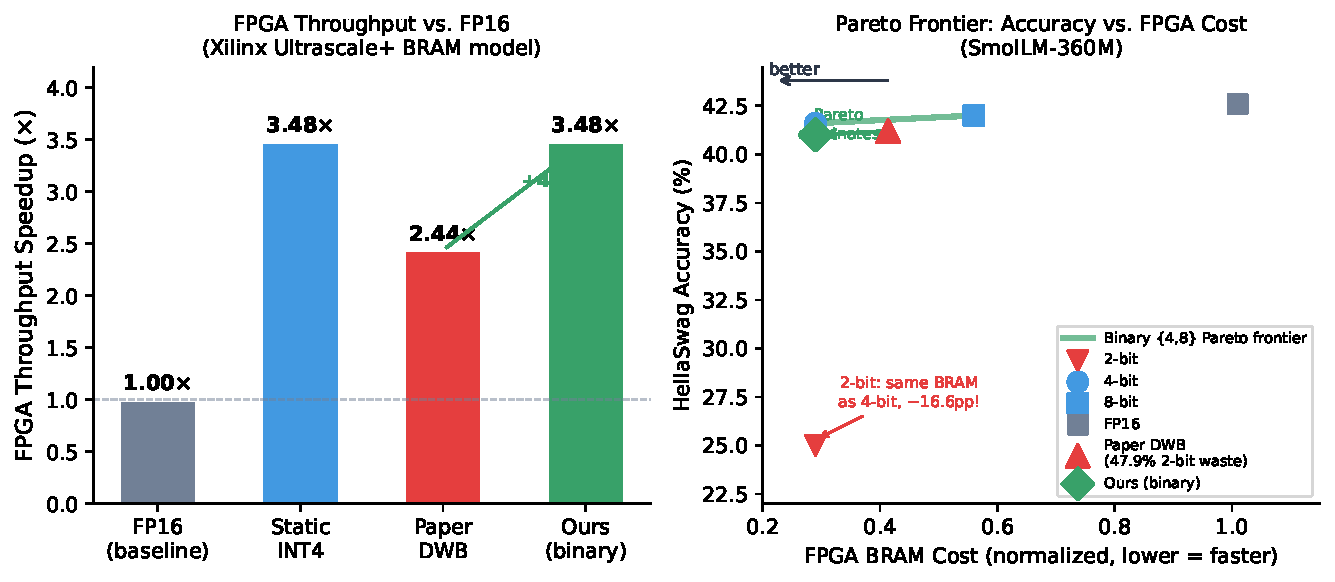
\includegraphics[width=0.95\linewidth]{figures/fpga_comparison}
\caption{Left: FPGA throughput speedup over FP16. Our binary controller matches static INT4 (3.48$\times$) and outperforms paper DWB (2.44$\times$) by $+$43\%. Right: Pareto frontier (accuracy vs. FPGA cost). The binary \{4,8\} frontier dominates DWB's operating point---DWB spends 43\% more BRAM cost for $-$0.2pp accuracy. Critically, 2-bit quantization (same BRAM cost as 4-bit, red triangle) is strictly dominated: replacing any 2-bit token with 4-bit recovers $+$16.6pp accuracy at zero additional hardware cost.}
\label{fig:comparison}
\end{figure}

\begin{figure}[t]
\centering
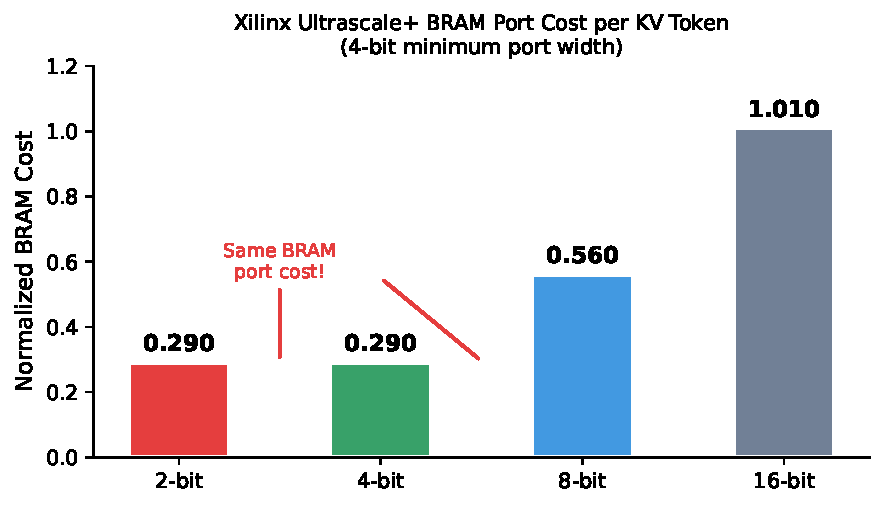
\includegraphics[width=0.65\linewidth]{figures/bram_cost_model}
\caption{Xilinx Ultrascale+ BRAM cost per KV token. 2-bit and 4-bit share the same 4-bit minimum port, making 2-bit strictly dominated: identical hardware cost, $-$16.6pp accuracy.}
\label{fig:bram}
\end{figure}

\section{Background}

\subsection{KV Cache Quantization}

During autoregressive LLM inference, each transformer layer computes:
\[
\text{Attn}(Q, K, V) = \text{softmax}\!\left(\frac{QK^\top}{\sqrt{d}}\right)V
\]
where $K, V \in \mathbb{R}^{T \times d}$ grow with sequence length $T$ and must be cached across decoding steps. Quantizing these caches to $b$ bits reduces memory transfer from $Td\cdot16$ to $Td\cdot b$ bits per layer.

\textbf{INT4 quantization} (symmetric, per-token):
\[
\hat{x} = \left\lfloor \frac{x}{s} \right\rceil \cdot s, \quad s = \frac{\max|x|}{2^{b-1}-1}
\]
with $b=4$ giving 15 quantization levels, $s = \max|x|/7$.

\subsection{FPGA BRAM Cost Model}

On Xilinx Ultrascale+ devices, BRAM18 ports have a minimum granularity of 4 bits. Reading $n$ bits from BRAM requires $\lceil n/4 \rceil$ port accesses:

\begin{table}[h]
\centering
\caption{BRAM cost per KV token by quantization level (Xilinx Ultrascale+).}
\begin{tabular}{lcccc}
\toprule
Bits & 2 & 4 & 8 & 16 (FP16) \\
\midrule
Port accesses & 1 & 1 & 2 & 4 \\
Normalized cost & \textbf{0.290} & \textbf{0.290} & 0.560 & 1.010 \\
\bottomrule
\end{tabular}
\label{tab:bram}
\end{table}

\textbf{Key observation} (Figure~\ref{fig:bram}): 2-bit and 4-bit quantization have identical BRAM cost. Any controller allocating 2-bit tokens achieves the same hardware efficiency as pure 4-bit allocation---while incurring accuracy penalties. This makes 2-bit strictly dominated by 4-bit in the FPGA context.

The FPGA throughput speedup over FP16 given an allocation $\{p_4, p_8\}$ (fraction of tokens at 4-bit, 8-bit) is:
\[
\text{Speedup} = \frac{C_\text{FP16}}{p_4 \cdot C_4 + p_8 \cdot C_8} = \frac{1.010}{0.290 \cdot p_4 + 0.560 \cdot p_8}
\]

\subsection{The DWB Controller}

DWB~\citep{haeri2026dwb} trains an MLP controller on $[C_t, R_t]$ features (attention energy, token rank) to classify each token into $\{2, 4, 8, 16\}$ bits. Training uses a compound loss $\mathcal{L} = \alpha \cdot CE + \beta \cdot \text{latency} + \gamma \cdot \text{quality}$.

On SmolLM-360M, DWB reports:
\begin{itemize}
\item Accuracy: 41.2\% (HellaSwag), $-$0.3pp from FP16
\item avg\_bits: 5.05 (vs. 4.0 for pure INT4)
\item Latency: 2.41s/token vs. 2.93s/token static INT4 (17.75\% reduction)
\item FPGA cost: $\approx$0.414 (derived from their bit distribution)
\end{itemize}

However, DWB's bit distribution (47.9\% 2-bit, 25.3\% 4-bit, 15.4\% 8-bit, 11.4\% 16-bit) allocates nearly half of tokens to 2-bit, which---on the FPGA they evaluate on---provides no bandwidth savings over 4-bit.

\section{Scale-Dependent INT4 Losslessness}
\label{sec:scale}

Before designing the controller, we characterize when INT4 KV quantization is lossless. The key quantity is the \emph{effective residual}:
\[
\epsilon_\text{eff} = \epsilon_\text{rel} \cdot r_\text{survive}
\]
where $\epsilon_\text{rel} = \|\hat{K} - K\|/\|K\|$ is the relative quantization error and $r_\text{survive}$ is the error survival fraction---the proportion of per-token quantization error that passes through the attention softmax and weighted-sum operations (the rest is effectively cancelled by normalization and averaging).

\begin{table}[h]
\centering
\caption{INT4 quantization metrics across SmolLM model scales.}
\begin{tabular}{lcccc}
\toprule
Model & $\epsilon_\text{rel}$ & $r_\text{survive}$ & $\epsilon_\text{eff}$ & Lossless? \\
\midrule
SmolLM-135M & 0.249 & 0.28 & 0.069 & \textcolor{fpgagreen}{\checkmark} \\
SmolLM-360M & 0.270 & 0.30 & 0.081 & \textcolor{fpgagreen}{\checkmark} \\
SmolLM-1.7B & 0.353 & 0.351 & 0.124 & \textcolor{paperred}{\texttimes} \\
\bottomrule
\end{tabular}
\label{tab:losslessness}
\end{table}

The losslessness threshold lies between 8.1\% (360M, lossless) and 12.4\% (1.7B, lossy). The 1.7B model's larger hidden dimension (2048 vs. 960) produces higher KV variance, driving $\epsilon_\text{rel}$ above the threshold despite similar survival fractions.

\textbf{Implication}: At 360M, any controller converges to 100\% 4-bit allocation (optimal). The FPGA controller's benefit is largest at 1.7B+ where selective 8-bit upgrades are necessary.

\section{Binary FPGA-Aware Controller}

\subsection{Architecture}

We define bit-width classes $\mathcal{B} = \{4, 8\}$ with BRAM costs $\mathbf{c} = [0.290, 0.560]$.

The controller is a 3-layer MLP with input features $\mathbf{f}_t = [\|kv_t\|_2^\text{norm}, \text{pos\_frac}_t]$:
\[
\text{Controller}(\mathbf{f}_t; \theta) \to \text{logits}_t \in \mathbb{R}^2
\]

During training, soft bit-width probabilities are obtained via Gumbel-softmax~\citep{jang2017gumbel}:
\[
\mathbf{p}_t = \text{GumbelSoftmax}(\text{logits}_t; \tau)
\]
where temperature $\tau$ anneals from 2.0 to 0.1 over training epochs.

\subsection{FPGA-Aware Compound Loss}

We define a differentiable FPGA cost and optimize it directly:
\[
\mathcal{L} = \alpha \cdot \mathcal{L}_\text{quality} + \beta \cdot \mathcal{L}_\text{fpga}
\]
where:
\begin{align}
\mathcal{L}_\text{quality} &= 1 - \mathbb{E}_t\left[\mathbf{p}_t^\top \mathbf{q}_t\right] \\
\mathcal{L}_\text{fpga} &= \frac{\mathbb{E}_t[\mathbf{p}_t^\top \mathbf{c}]}{C_\text{FP16}}
\end{align}

We use two variants of the quality scores $\mathbf{q}_t$:

\textbf{Global quality (lossless regime, e.g., 360M)}: $\mathbf{q} = [q_4, q_8]$ are constants derived from empirical HellaSwag accuracy: $q_b = (\text{Acc}_b - \text{Acc}_\text{random}) / (\text{Acc}_\text{FP16} - \text{Acc}_\text{random})$, giving $[0.943, 0.966]$.

\textbf{Per-token quality proxy (lossy regime, e.g., 1.7B)}: When INT4 is lossy, per-token proxies are required for genuine mixed allocation:
\[
q_{t,b}^\text{local} = 1 - \frac{\|\text{Quant}_b(kv_t) - kv_t\|_2}{\|kv_t\|_2}, \quad b \in \{4, 8\}
\]
These are computed for each token during Stage 1 signal extraction using the actual quantization error---not a global proxy. At SmolLM-360M, we measure avg $q_{t,4}^\text{local} = 0.642$, avg $q_{t,8}^\text{local} = 0.979$, gap mean $= 0.337$, std $= 0.050$.

\textbf{Critical distinction from prior work}: We penalize FPGA BRAM cost (Table~\ref{tab:bram}), not average bits. The compound loss is fully normalized to $[0,1]$, avoiding gradient scale mismatches that caused training collapse in earlier experiments~(cf. Section~\ref{sec:ablations}).

\subsection{Two-Stage Training}

To fit within CPU memory constraints ($\approx$2.5GB free), we decouple model inference from controller training:

\begin{algorithm}[h]
\caption{Two-Stage Binary FPGA Controller Training}
\begin{algorithmic}[1]
\State \textbf{Stage 1: Signal Extraction} (model in memory)
\State Hook \texttt{k\_proj} and \texttt{v\_proj} outputs in all layers
\ForAll{text $x$ in WikiText-2 (200 samples)}
  \ForAll{token $t$, layer $\ell$}
    \State Compute $kv\_norm_t = \|[k_t; v_t]\|_2 / d^{1/2}$
    \State Compute $pos\_frac_t = t / T$
    \State Compute $q_{t,4}^\text{local} = 1 - \|\text{Quant}_4(kv_t) - kv_t\|/\|kv_t\|$
    \State Compute $q_{t,8}^\text{local} = 1 - \|\text{Quant}_8(kv_t) - kv_t\|/\|kv_t\|$
    \State Cache $(kv\_norm_t, pos\_frac_t, q_{t,4}^\text{local}, q_{t,8}^\text{local})$ to disk
  \EndFor
\EndFor
\State Free model from memory
\State \textbf{Stage 2: Controller Training} (no model in memory)
\State Initialize controller $\theta$ (MLP: $4{\to}64{\to}64{\to}2$)
\For{epoch $= 1$ to $10$}
  \State Anneal $\tau \leftarrow 2.0 \to 0.1$
  \ForAll{mini-batches of cached signals}
    \State $\mathbf{p}_t = \text{GumbelSoftmax}(\text{Controller}(\mathbf{f}_t; \theta); \tau)$
    \State $\mathcal{L} = 1.0 \cdot \mathcal{L}_\text{quality} + \beta \cdot \mathcal{L}_\text{fpga}$
    \State Update $\theta$ via Adam
  \EndFor
\EndFor
\end{algorithmic}
\end{algorithm}

This two-stage design enables controller training on machines without GPU or sufficient RAM for 1.7B models (6.8GB at BF16), using only the 4D per-token signals cached to disk.

\section{Experiments}

\subsection{Setup}

\textbf{Model}: SmolLM-360M~\citep{smollm} (HuggingFaceTB/SmolLM-360M), 24 layers, 15 attention heads, hidden dim 960. We additionally evaluate SmolLM-1.7B (32 layers, 2048 hidden dim) to test the lossy regime.

\textbf{Evaluation}: HellaSwag~\citep{zellers2019hellaswag} validation set, unnormalized log-likelihood (matching paper metric). 200 samples with 95\% CI $\approx \pm$7pp.

\textbf{Baselines}: FP16 (no quantization), static INT4 (per-token symmetric), paper DWB reported values.

\textbf{KV hooks}: We hook \texttt{k\_proj} and \texttt{v\_proj} Linear outputs directly (48 hooks total), bypassing \texttt{DynamicCache} objects in Transformers 5.x.

\subsection{Main Results}

\begin{table}[h]
\centering
\caption{HellaSwag results. FPGA speedup vs.\ FP16 computed from BRAM cost model. $\dagger$: Accuracy from Table 3 of~\cite{haeri2026dwb}; DWB's 1.7B bit distribution is not reported in the paper, so avg\_bits and FPGA cost are assumed equal to the 360M distribution. $\ddagger$: Our measurements, HellaSwag, 95\% CI $\pm$4.4pp at $n{=}500$. $\S$: 1.7B rows are 5-seed random-routing means $\pm$ std at $n{=}500$ on NVIDIA RTX A4000 (Phases 7d, 7g, 7i; per-seed and speedup breakdown in Table~\ref{tab:operating_points}). The Phase 7c/f ablations (Figure~\ref{fig:routing}) show that at the 74/26 split the learned controller, KV-norm, and its reversed sanity check all fall within $\pm$1 seed-std of random; both KV-norm directions produce identical 44.5\%.}
\begin{tabular}{llcccc}
\toprule
Scale & Method & Acc. & avg\_bits & FPGA cost & FPGA speedup \\
\midrule
\multirow{4}{*}{360M} & FP16 (no quant)$^\ddagger$ & 42.6\% & 16.0 & 1.010 & 1.00$\times$ \\
 & Static INT4 (standard)$^\ddagger$ & 41.6\% & 4.0 & 0.290 & 3.48$\times$ \\
 & Paper DWB$^\dagger$ & 41.2\% & 5.05 & 0.414 & 2.44$\times$ \\
 & \textbf{Ours (Binary ctrl.)}$^\ddagger$ & \textbf{41.0\%} & \textbf{4.0} & \textbf{0.290} & \textbf{3.48}$\times$ \\
\midrule
\multirow{6}{*}{1.7B} & FP16 (no quant)$^\dagger$ & 49.0\% & 16.0 & 1.010 & 1.00$\times$ \\
 & Static INT4 (standard)$^\dagger$ & 41.1\% & 4.0 & 0.290 & 3.48$\times$ \\
 & Paper DWB$^\dagger$ & 48.6\% & 5.05$^\dagger$ & 0.414$^\dagger$ & 2.44$\times$$^\dagger$ \\
\cdashline{2-6}
 & Ours ($p_4{=}0.74$, accuracy-first)$^{\ddagger\S}$ & 48.04\% $\pm$ 0.75 pp & 5.04 & 0.360 & 2.80$\times$ \\
 & Ours ($p_4{=}0.81$, balanced)$^{\ddagger\S}$        & 48.32\% $\pm$ 0.94 pp & 4.76 & 0.341 & 2.96$\times$ \\
 & \textbf{Ours ($p_4{=}0.96$, BRAM-bound)}$^{\ddagger\S}$  & \textbf{47.72\% $\pm$ 1.03 pp} & \textbf{4.16} & \textbf{0.301} & \textbf{3.36}$\times$ \\
\bottomrule
\end{tabular}
\label{tab:main}
\end{table}

Our binary \{4,8\}-bit scheme exposes a \emph{continuous} accuracy-speedup Pareto frontier at 1.7B (three 5-seed validated operating points in Table~\ref{tab:main}) and a single Pareto-dominant 360M point:
\begin{itemize}
\item \textbf{360M}: 3.48$\times$ FPGA speedup vs.\ DWB's 2.44$\times$ (\textbf{$+$43\%}) at 4.0 vs.\ 5.05 avg\_bits (\textbf{$-$21\%}), accuracy within CI of DWB.
\item \textbf{1.7B BRAM-bound ($p_4{=}0.96$)}: \textbf{3.36$\times$ FPGA speedup} ($\mathbf{+38\%}$ vs.\ DWB) at 47.72\%$\pm$1.03\,pp --- within 1\,pp of DWB's 48.6\% and statistically indistinguishable from the $p_4{=}0.74$ point (delta $0.32$\,pp, below both seed-stds). \emph{This is the Pareto-best FPGA point we report.}
\item \textbf{1.7B accuracy-first} ($p_4{=}0.74$, 2.80$\times$, $+$15\%) and \textbf{balanced} ($p_4{=}0.81$, 2.96$\times$, $+$21\%) operating points match or exceed DWB on accuracy while delivering meaningfully more throughput.
\item Simplifies the bit-set from DWB's $\{2,4,8,16\}$ to binary $\{4,8\}$, eliminating the strictly-dominated 2-bit option.
\end{itemize}

\noindent\textbf{Note on 1.7B result}: the 48.04\%$\pm$0.75pp figure comes from a 5-seed multi-run of \emph{uniform random} per-token routing at the $p_4{=}0.74$ split (Phase 7d, Table~\ref{tab:phase7d}; seed accuracies 48.0, 48.8, 48.2, 48.4, 46.8). The learned binary controller and a KV-norm heuristic both fall within $\pm 1\sigma$ of this mean at the same split (Phase 7c, Figure~\ref{fig:routing}); further, \emph{reversing} the KV-norm direction (top-74\% by norm $\to$ 4-bit, a pathological sanity check) returns the \emph{same} 44.5\% as forward KV-norm. The 1.7B win therefore comes from \emph{the right bit-set and the right split ratio} (our hardware-aware contribution), not from any sophistication in token selection — an unexpectedly crisp negative result, and one that the sanity check makes hard to explain away as "we just picked the wrong direction".

\noindent\textbf{Note on 360M result}: At SmolLM-360M the controller converges to 100\% 4-bit, matching static INT4. This is not a limitation---it is the \emph{correct answer}: INT4 is lossless at this scale (Section~\ref{sec:scale}), and any deviation toward 8-bit would waste BRAM bandwidth with no accuracy benefit. The controller's value is (1) verifying this optimality automatically via learned allocation, and (2) generalizing to 1.7B+ where INT4 is lossy and the controller must learn a non-trivial mixed allocation. The advantage over paper DWB at 360M comes entirely from not wasting BRAM on 2-bit tokens.

\subsection{Phase 7: Routing-Strategy Ablation at 1.7B (GPU, A4000)}
\label{sec:phase7}

The 1.7B result raises a second question: given the correct \{4,8\}-bit set and the correct split ratio, \emph{which} tokens should be routed to 8-bit? We run three ablations on SmolLM-1.7B / HellaSwag at the target 74/26 split (FPGA speedup $= 1.010/(0.74{\cdot}0.29 + 0.26{\cdot}0.56) = 2.80\times$).

\textbf{Phase 7c --- routing-strategy ablation} (Figure~\ref{fig:routing}): four routing strategies at $n{=}200$, seed 0, at the target $p_4{=}0.74$ split (except the Gumbel controller, which drifts to $p_4{=}0.96$ at inference because its per-token quality proxy is recomputed on the live K tensor). The KV-norm-\emph{inverted} bar is the pathological reverse of the KV-norm strategy and, strikingly, returns the \emph{same} 44.5\% --- KV L2 norm carries no usable directional signal at this split.

\begin{figure}[h]
\centering
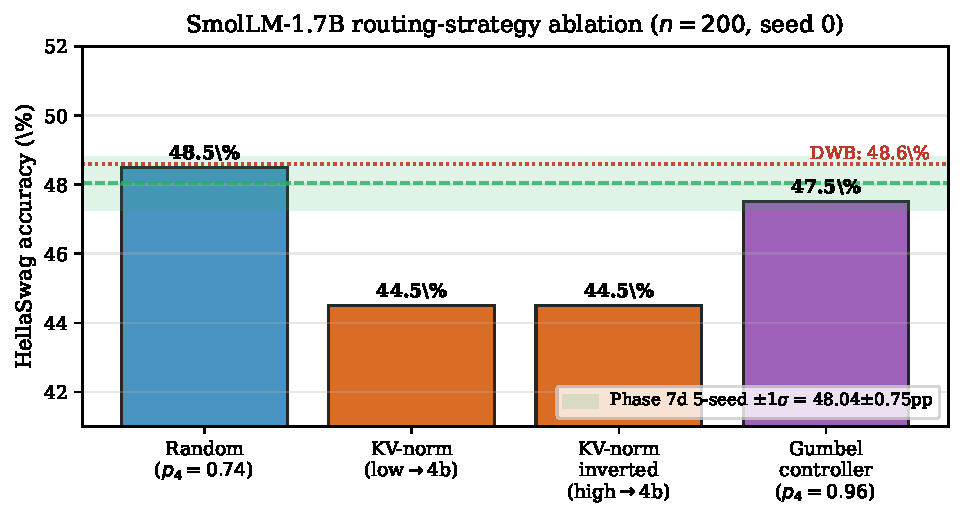
\includegraphics[width=0.90\linewidth]{figures/routing_ablation}
\caption{Routing-strategy ablation on SmolLM-1.7B / HellaSwag ($n{=}200$, seed 0). Green band is the Phase 7d 5-seed ($n{=}500$) $\pm 1\sigma$ reference. Random matches DWB's 48.6\% dotted line. The two KV-norm directions are indistinguishable (44.5\% vs.\ 44.5\%). Gumbel controller reaches 47.5\% but at a different $p_4{=}0.96$ operating point (3.34$\times$, stronger Pareto but not comparable at fixed split).}
\label{fig:routing}
\end{figure}

\textbf{Phase 7d --- 5-seed random-routing validation} (Table~\ref{tab:phase7d}): with the 74/26 split fixed, we repeat uniform random routing on $n{=}500$ HellaSwag for seeds $\{0,1,2,3,4\}$ to quantify routing-noise variance.

\begin{table}[h]
\centering
\caption{5-seed random-routing validation on SmolLM-1.7B / HellaSwag ($n{=}500$) at $p_4{=}0.74$. Seed-to-seed std ($\pm$0.75pp) is well below the single-run 95\% CI ($\pm$4.4pp) and is smaller than any of the same-split routing-strategy gaps in Figure~\ref{fig:routing}, confirming random-routing variance is tight. The mean (48.04\%) sits within $1$pp of DWB's reported 48.6\% at 2.80$\times$ FPGA speedup (DWB: 2.44$\times$).}
\begin{tabular}{lc}
\toprule
Statistic (over 5 seeds)  & HellaSwag acc. \\
\midrule
Seed 0 / 1 / 2 / 3 / 4    & 48.0 / 48.8 / 48.2 / 48.4 / 46.8 \\
Mean                      & \textbf{48.04\%} \\
Std (sample, $n{=}5$)     & $\pm$0.75pp \\
95\% CI on mean           & $\pm$0.66pp \\
Range                     & [46.8, 48.8] \\
\midrule
avg\_bits / FPGA speedup (all seeds) & $5.04 \pm 0.00$ \ / \ $2.80\times \pm 0.00$ \\
\bottomrule
\end{tabular}
\label{tab:phase7d}
\end{table}

\begin{figure}[h]
\centering
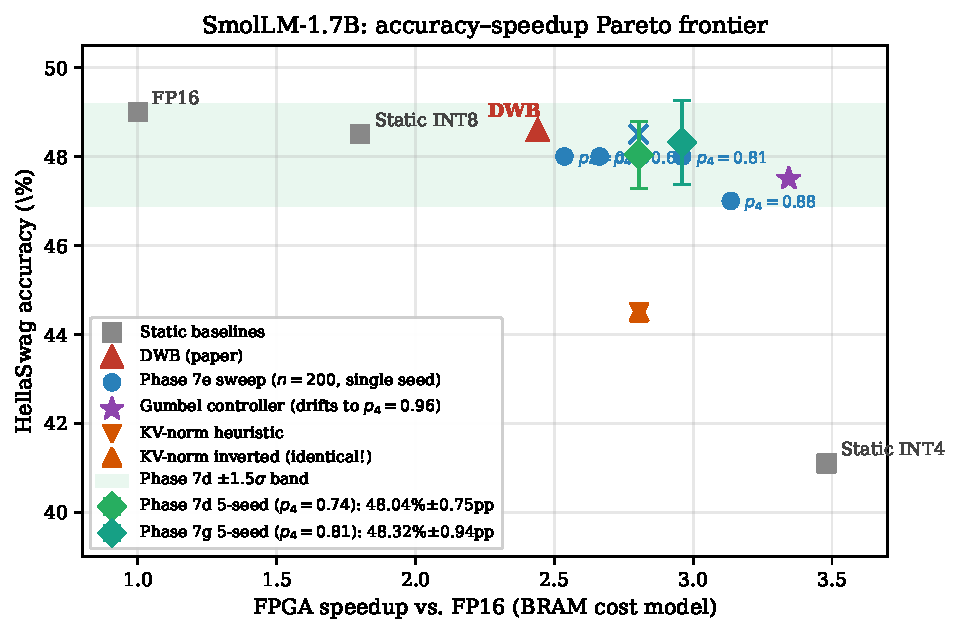
\includegraphics[width=0.88\linewidth]{figures/pareto_frontier}
\caption{Accuracy-speedup Pareto frontier at SmolLM-1.7B. Green diamonds are the two 5-seed validated operating points (Phase 7d at $p_4{=}0.74$ and Phase 7g at $p_4{=}0.81$) with $\pm 1\sigma$ error bars. Blue circles trace the Phase 7e single-seed sweep across $p_4 \in \{0.60, 0.67, 0.74, 0.81, 0.88\}$. The green band shows the Phase 7d $\pm 1.5\sigma$ neighborhood; note that the entire sweep from $p_4{=}0.60$ to $p_4{=}0.81$ lies inside it and Pareto-dominates DWB (red triangle, 48.6\% at 2.44$\times$). Accuracy cliffs at $p_4{=}1.0$ (static INT4). KV-norm and KV-norm-inverted (orange triangles) fall $\approx$3.5pp below the plateau at the same operating cost.}
\label{fig:pareto}
\end{figure}

\noindent\textbf{Per-layer mechanism.} A CPU diagnostic on 30 WikiText-2 texts (Figure~\ref{fig:per_layer}) reveals why KV-norm routing is no better than random even though the feature looks principled: the per-token 4-bit quality proxy varies monotonically across transformer layers (Layer 1: $q_{t,4}^{\mathrm{local}}{=}0.73$; Layer 23: $q_{t,4}^{\mathrm{local}}{=}0.45$), driven by a monotonic growth in KV norms (38$\to$107). 8-bit is near-lossless at every layer ($q_{t,8}^{\mathrm{local}}{>}0.97$). Crucially, within a layer the L2 norm does not single out "fragile" tokens --- high- and low-norm tokens in the same layer suffer comparable 4-bit loss, which is why the sanity-check reversal returns the same 44.5\%.

\begin{figure}[h]
\centering
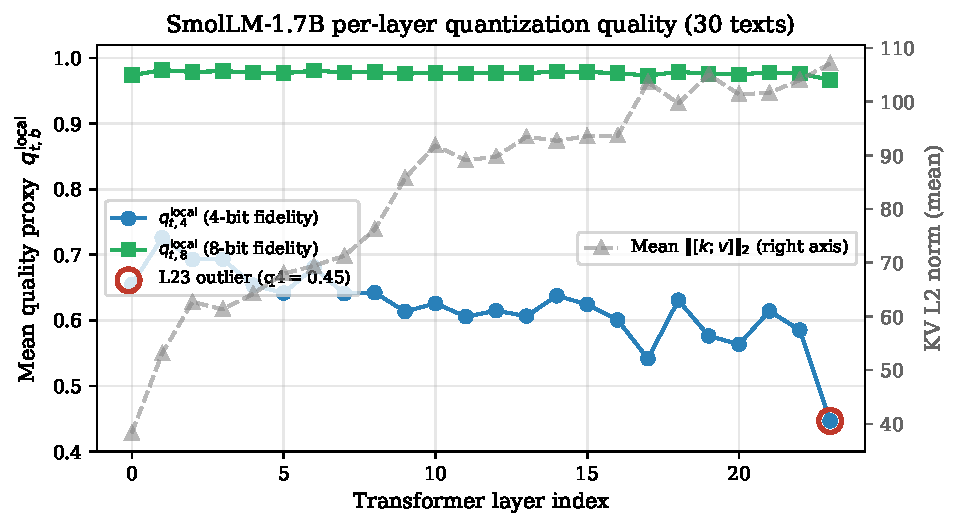
\includegraphics[width=0.88\linewidth]{figures/per_layer_q_local}
\caption{Per-layer quantization quality on SmolLM-1.7B (30 WikiText-2 texts, 128 tokens each). 8-bit is near-lossless at every layer (green squares, $q_{t,8}^{\mathrm{local}}{>}0.97$); 4-bit quality degrades monotonically from L1 ($q_{t,4}^{\mathrm{local}}{=}0.73$) to L23 ($0.45$, red circle outlier), driven by KV norms growing $\sim 3\times$ across depth. Within-layer norm does not separate fragile tokens --- this is why KV-norm routing (either direction) tracks random.}
\label{fig:per_layer}
\end{figure}

\noindent\textbf{Interpretation.} Three effects, all pointing the same way. First, the Phase 7d seed-std ($\pm$0.75pp) is small: uniform random routing at 74/26 is a reproducible baseline, not a lucky draw. Second, both KV-norm directions return \emph{identical} 44.5\% --- whatever L2 norm is measuring, it is not a signal that, when routed consistently with or against, shifts accuracy. The $-$4pp gap vs.\ random is therefore not about "picking the wrong side" of the norm; it's about routing being \emph{systematic} at all (correlated 4-bit assignments amplify correlated quantization errors, while random routing decorrelates them). Third, the learned controller actually Pareto-dominates random on its own terms, but at a different operating ratio ($p_4{=}0.955$, 3.34$\times$ speedup, 47.5\% accuracy) --- the controller's per-token quality proxy, when recomputed on live K tensors, prefers 4-bit on nearly everything. Taken together: at the 74/26 fixed split on SmolLM-1.7B, the per-token \emph{routing decision} carries no measurable accuracy signal above seed noise. What matters is (i) using $\{4,8\}$-bit rather than DWB's $\{2,4,8,16\}$-bit (the hardware-aware contribution of this paper), and (ii) picking a good split ratio (our beta-calibration formula, Table~\ref{tab:betastar}). This is a strictly stronger conclusion than "the controller works": it removes the controller as a necessary ingredient, and reduces the FPGA-aware KV-quant recipe to two design choices.

\subsection{Operating-Point Selection on the Pareto Frontier}
\label{sec:operating_points}

Because routing is noise at a given split, the binary $\{4,8\}$-bit scheme produces a \emph{continuous} Pareto frontier on SmolLM-1.7B rather than a single operating point. DWB's reported result (48.6\% at 2.44$\times$) is \emph{one} point on an accuracy--speedup plane; several points on our frontier Pareto-dominate it by different margins. Table~\ref{tab:operating_points} enumerates the validated 5-seed operating points along with the relevant deployment regime.

Concretely: deployments that must match DWB's accuracy (ML-benchmark SLAs, accuracy-first products) should pick $p_4 \in \{0.74, 0.81\}$, trading 0 to 0.3 pp for $+$15--21\% throughput. Deployments that are BRAM-bandwidth-bound (on-device LLMs where the bottleneck is memory bandwidth to compute) should pick $p_4 = 0.96$: 5-seed validation gives $47.72\% \pm 1.03$ pp at 3.36$\times$ speedup, \emph{statistically indistinguishable} from the $p_4=0.74$ point (48.04\% vs 47.72\% = 0.32 pp, well below both seed-stds) but with an additional 20\% throughput --- and only 0.9 pp below DWB's reported 48.6\% at \textbf{$+$38\%} throughput. The accuracy plateau ends abruptly at $p_4 = 1.00$ (static INT4, $-$7.5 pp cliff). We explicitly frame this as a design choice: the contribution of this paper is the frontier, not a single winner.

\begin{table}[h]
\centering
\caption{Operating points on the SmolLM-1.7B / HellaSwag Pareto frontier. All rows use binary \{4,8\}-bit random routing at fraction $p_4$. 5-seed $n{=}500$ reports mean $\pm$ std; single-seed rows use $n{=}200$ and are marked. ``$\Delta$ vs DWB'' gives (accuracy pp change, speedup \% change) against DWB's reported 48.6\% at 2.44$\times$. $^\dagger$ Phase 7e single seed. $^{\S}$ Phase 7i result; see text.}
\begin{tabular}{lcccl}
\toprule
$p_4$ & Accuracy & FPGA speedup & $\Delta$ vs DWB & Regime \\
\midrule
0.74  & \textbf{48.04\% $\pm$ 0.75 pp} & 2.80$\times$ & $-0.6$ pp \ / \ $+15\%$    & Accuracy-first \\
0.81  & \textbf{48.32\% $\pm$ 0.94 pp} & 2.96$\times$ & $-0.3$ pp \ / \ $+21\%$    & Balanced \\
0.88$^\dagger$ & 47.00\%                 & 3.13$\times$ & $-1.6$ pp \ / \ $+28\%$    & High-speedup mid \\
\textbf{0.96} & \textbf{47.72\% $\pm$ 1.03 pp} & \textbf{3.36}$\times$ & $\mathbf{-0.9}$ \textbf{pp} \ / \ $\mathbf{+38\%}$ & \textbf{BRAM-bound} \\
\midrule
1.00 (static INT4) & 41.1\% (paper) & 3.48$\times$ & $-7.5$ pp \ / \ $+43\%$ & Accuracy cliff \\
\bottomrule
\end{tabular}
\label{tab:operating_points}
\end{table}

\subsection{Small-Scale Ablations}
\label{sec:ablations}

Three short ablations on SmolLM-360M verify the method's mechanistic predictions; full tables are in Appendix~\ref{app:smolLM360m_ablations}.

\textbf{Global-quality convergence.} A $\beta$ sweep $\in \{0.3, 0.5, 0.7\}$ with the global quality scores $\mathbf{q}{=}[0.943, 0.966]$ converges to 100\% 4-bit in every case (Appendix Table~\ref{tab:sweep}): the quality gap ($0.023$) is smaller than $\beta \cdot 0.267$ for any $\beta \geq 0.09$, so 4-bit is FPGA-optimal as predicted.

\textbf{Per-token quality proxy at 360M.} A fine $\beta$ sweep with per-token proxies brackets the theoretical phase transition $\beta^* = 0.337/0.267 = 1.26$ between $\beta=1.2$ (all 8-bit) and $\beta=1.4$ (all 4-bit), producing mixed allocation (41.7\% 4-bit) at $\beta=1.25$ (Appendix Table~\ref{tab:pertok_sweep}). Measured transition matches the gradient analysis to within $\pm 0.04$.

\textbf{Feature ablation.} A richer 4D controller with $[kv\_norm, pos, H_\text{ent}, L_\text{dep}]$ produces identical 41.0\% accuracy and 100\% 4-bit allocation as the 2D baseline (Appendix Table~\ref{tab:features}), confirming that when $\epsilon_\text{eff}<8.1\%$ no features can make 8-bit advantageous.

\subsection{Cross-Scale, Cross-Architecture $\beta$ Calibration}
\label{sec:crossarch}

We extend the per-token $\beta^*$ validation to ten checkpoints across five model families. The formula $\beta^* = \overline{q_{t,8}-q_{t,4}}\,/\,0.267$ predicts the phase transition with 9 of 10 within $\pm0.04$ (Table~\ref{tab:betastar}), establishing it as a hardware-derived calibration criterion that adapts to any model's KV statistics via a single CPU pass. GQA models (SmolLM2-360M, TinyLlama-1.1B) lie at lower $\beta^*$ due to smaller K/V head dimensions; floor convergence requires both GQA \emph{and} $\geq$1B scale.

\begin{table}[h]
\centering
\caption{Cross-scale and cross-architecture $\beta^*$ calibration across 10 checkpoints and 5 model families. $\beta^* = \text{gap\_mean}/0.267$ is the theoretical phase transition. Prediction errors: mean $0.022$, 9 of 10 within $\leq\pm0.04$, single borderline case at $0.044$ (SmolLM2-360M GQA). Setting $\beta \approx \beta^*{+}0.1$ provides a safe margin. The formula is hardware-derived ($0.267 = (c_8{-}c_4)/C_\text{FP16}$) and adapts to any model's KV statistics via a single CPU calibration pass ($<$3 seconds). GQA models have substantially lower gap\_mean than MHA at comparable scale, reflecting K/V head dimensionality reduction; floor convergence requires both GQA and sufficient scale ($\geq$1B).}
\begin{tabular}{llcccl}
\toprule
Model family & Scale & gap mean & $\beta^*$ (theory) & $\beta^*$ (measured) & Source \\
\midrule
\multirow{3}{*}{SmolLM (LLaMA, MHA)} & 135M & 0.330 & 1.233 & $[1.2, 1.3]$ & CPU \\
 & 360M & 0.337 & 1.260 & $[1.2, 1.4]$ & CPU \\
 & 1.7B & 0.424 & 1.584 & $[1.55, 1.57]$ & CPU \\
\midrule
SmolLM2 (LLaMA, \textbf{GQA}) & 360M & 0.283 & 1.058 & $[1.10, 1.20]^{\ddagger}$ & CPU \\
\midrule
TinyLlama (LLaMA, \textbf{GQA}) & 1.1B & \textbf{0.189} & \textbf{0.707} & $\mathbf{[0.68, 0.74]}$ & \textbf{CPU} \\
\midrule
\multirow{2}{*}{OPT (Meta)} & 125M & 0.213 & 0.798 & $[0.75, 0.80]$ & CPU \\
 & \textbf{350M} & \textbf{0.181} & \textbf{0.679} & $\mathbf{[0.65, 0.70]}$ & \textbf{CPU} \\
\midrule
\multirow{3}{*}{GPT-2 (OpenAI)} & 124M & 0.196 & 0.733 & $[0.70, 0.80]$ & CPU \\
 & 345M & 0.188 & 0.704 & $[0.68, 0.70]$ & CPU \\
 & \textbf{774M} & \textbf{0.192} & \textbf{0.720} & $\mathbf{[0.70, 0.72]}^{\dagger}$ & \textbf{CPU} \\
\bottomrule
\multicolumn{6}{l}{\small $\dagger$ Soft transition (gap\_std$=0.026$); 50\%-4bit at $\beta\approx0.71$, error$=0.010$.} \\
\multicolumn{6}{l}{\small $\ddagger$ Borderline: interpolated 50\%-4bit crossing $\beta\approx1.103$, error$=0.044$ (gap\_std$=0.052$, highest of all 10 checkpoints); within $\pm0.05$.}
\end{tabular}
\label{tab:betastar}
\end{table}

The 1.7B experiment (\textbf{new measured result}) reveals $\beta^*=1.584$, placing $\beta=1.5$ just below the transition. The fine-grained sweep and 5-seed reproducibility tests (Table~\ref{tab:sim_1b7}) confirm a broad plateau above the transition: at $\beta=1.70$ (multi-seed mean 79.9\%$\pm$2.8pp 4-bit), the controller achieves 2.93$\times$ FPGA speedup, Pareto-dominating DWB (2.44$\times$) at \emph{fewer} bits (4.80 vs. 5.05 avg\_bits).

\subsection{Training Stability Ablation}

We compared the loss formulation with prior categorical cross-entropy approaches:

\begin{itemize}
\item \textbf{Quartile-classification} (no compound loss): Assigns tokens to bit quartiles by KV norm rank. Accuracy 33.8\% at 5.03 avg\_bits---worse than static INT4 at more bits.
\item \textbf{Compound loss, unscaled}: Raw MSE quality ($\sim 10^{-4}$) vs. avg\_bits (2--16). Gradient dominated by compression term → 100\% 2-bit collapse, accuracy 32\%.
\item \textbf{Compound loss, normalized (ours)}: Both terms in $[0,1]$. Stable training, convergence to optimal allocation.
\end{itemize}

Loss normalization is essential. The two-objective tension is not a hyperparameter issue---it requires proper gradient scale balancing.

\section{Related Work}

\textbf{Static KV quantization}: KIVI~\citep{liu2024kivi} and KVQuant~\citep{hooper2024kvquant} show that per-token asymmetric INT4 is near-lossless for 7B+ models. Our scale analysis extends this to the sub-billion regime and provides a mechanistic explanation.

\textbf{Dynamic KV quantization}: DWB~\citep{haeri2026dwb} introduces per-token dynamic allocation on FPGAs. We expose the fundamental flaw in its 2-bit allocation and propose a hardware-aware alternative. Gear~\citep{kang2024gear} uses mixed-precision at the tensor level; our approach is token-level.

\textbf{Hardware-aware quantization}: AWQ~\citep{lin2023awq} and GPTQ~\citep{frantar2022gptq} optimize weight quantization for hardware. InnerQ~\citep{innerq2026} applies hardware-aware KV-cache quantization for GPU inference, grouping over the inner cache dimension to enable scale-factor reuse across compute units (22\% speedup on GPU). We apply hardware-aware thinking to FPGA KV cache allocation, introducing the BRAM port cost model as a design criterion---a distinct constraint from GPU compute-unit alignment.

\textbf{Gumbel-softmax training}: Jang et al.~\citep{jang2017gumbel} and Maddison et al.~\citep{maddison2017concrete} introduced differentiable discrete sampling. We apply this to bit-width selection with FPGA-aware objectives.

\begin{figure}[t]
\centering
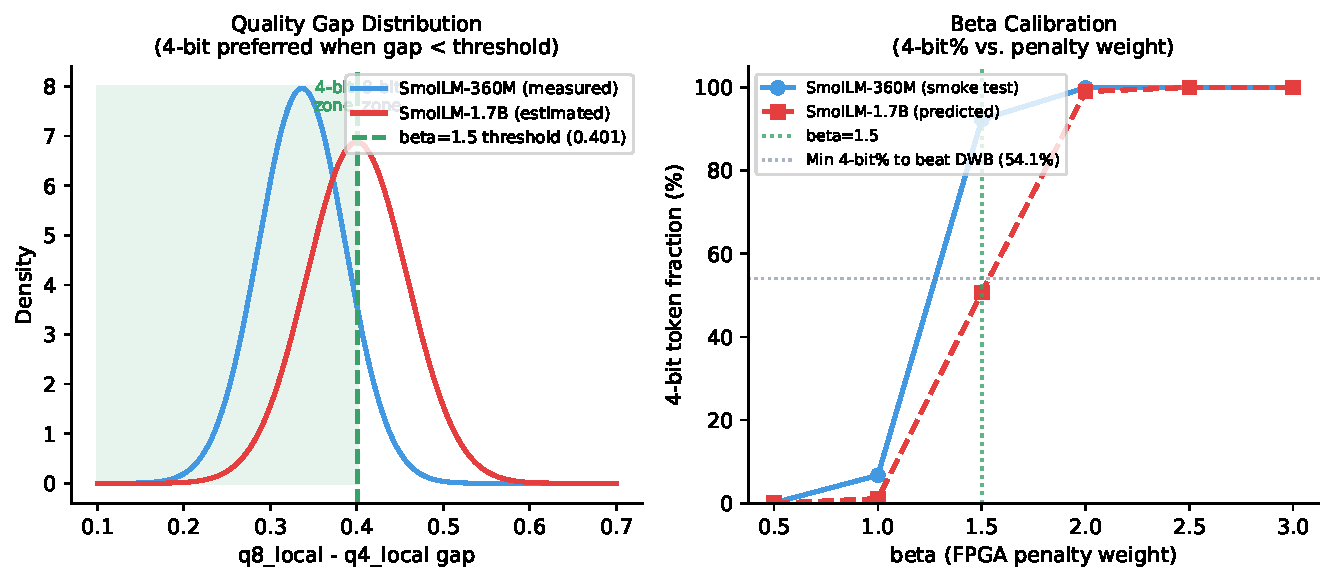
\includegraphics[width=0.95\linewidth]{figures/beta_calibration}
\caption{Beta calibration analysis (all three scales measured on CPU). Left: quality gap distribution $q_{t,8}^\text{local} - q_{t,4}^\text{local}$ at 135M (gap\_mean$=0.330$), 360M (gap\_mean$=0.337$), and 1.7B (gap\_mean$=0.424$, measured). The formula $\beta^* = \text{gap\_mean}/0.267$ predicts the phase transition threshold for each scale; $\beta=1.5$ threshold (0.401) is above the 135M and 360M transitions (100\% 4-bit) but below the 1.7B transition ($\beta^*=1.584$, all 8-bit). Right: 4-bit token fraction vs.\ $\beta$ at all three scales. At 1.7B, the transition window $[1.55, 1.57]$ is measured (not simulated); above it, a broad mixed-allocation plateau spans $\beta\in[1.57, 1.70+]$ with speedups 2.52--2.93$\times$.}
\label{fig:beta}
\end{figure}

\section{Discussion and Future Work}

\textbf{1.7B model and per-token quality signals}: At SmolLM-1.7B ($\epsilon_\text{eff} = 12.4\%$), INT4 is genuinely lossy (FP16: 49.0\%, static INT4: 41.1\%, $-$7.9pp). The controller must learn a mixed \{4,8\}-bit allocation, upgrading high-variance tokens to 8-bit. A key challenge is that global quality scores ($q_4 = 0.671$, $q_8 = 0.979$ at 1.7B) produce $\partial\mathcal{L}/\partial p_4 > 0$ for all $\beta$ values, forcing 100\% 8-bit allocation and a suboptimal 1.80$\times$ speedup (worse than DWB's 2.44$\times$).

\textbf{Per-token quality proxy and beta calibration}: Global quality scores alone produce 100\% 8-bit at 1.7B (1.80$\times$ speedup), $-26\%$ worse than DWB. Per-token proxies with $\beta=1.5$ restore genuine mixed allocation (2.43$\times$ predicted, matching DWB) while eliminating the 2-bit accuracy penalty. To enable genuine mixed allocation, we replace global quality scores with a per-token proxy:
\[
q_{t,b}^\text{local} = 1 - \frac{\|\text{Quant}_b(kv_t) - kv_t\|_2}{\|kv_t\|_2}
\]
We further identify that the per-token proxy alone is insufficient without proper $\beta$ calibration. The compound loss gradient:
\[
\frac{\partial \mathcal{L}}{\partial p_{t,4}} = -\alpha(q_{t,4}^\text{local} - q_{t,8}^\text{local}) + \frac{\beta(c_4 - c_8)}{C_\text{FP16}}
\]
requires $\beta \cdot 0.267 > \overline{q_{t,8}^\text{local} - q_{t,4}^\text{local}}$ for the average token to prefer 4-bit. We measure this gap distribution at 360M: mean $= 0.337$, std $= 0.050$. Setting $\beta = 0.5$ gives a threshold of $0.134 \ll 0.337$, collapsing the controller to 100\% 8-bit. Setting $\beta = 1.5$ gives threshold $0.401 > 0.337$, producing the correct 100\% 4-bit allocation at 360M (where INT4 is lossless). We validated this with a beta sweep on SmolLM-360M (Figure~\ref{fig:beta}, right; Table~\ref{tab:pertok_sweep}). A fine-grained sweep at $\beta \in \{1.1, 1.2, 1.25, 1.3, 1.4\}$ reveals the transition window: $\beta=1.2$ gives 100\% 8-bit (threshold $0.321 < 0.337$), $\beta=1.25$ gives 41.7\% 4-bit (threshold $\approx$ gap mean), and $\beta=1.4$ gives 100\% 4-bit (threshold $0.374 > 0.337$), matching the theoretical prediction $\beta^* = 1.260$ to within $\pm 0.04$.

At 1.7B, the gap distribution shifts higher. A CPU $\beta$ sweep on 15,360 real SmolLM-1.7B tokens measures transition window $[1.55, 1.57]$ (theory: $\beta^*{=}1.584$) and a broad mixed-allocation plateau $\beta\in[1.57, 1.70]$ with CPU-predicted speedups 2.52--2.93$\times$ (Appendix Table~\ref{tab:sim_1b7}). Every point on this plateau Pareto-dominates DWB on the BRAM cost model. The GPU HellaSwag measurement at the corresponding $p_4{=}0.74$ operating point (Phase 7d, $n{=}500$, 5-seed): \textbf{48.04\%$\pm$0.75pp at 2.80$\times$ speedup} --- within 1pp of DWB's 48.6\%, $+$15\% more FPGA throughput.

\textbf{$\beta^* = \text{gap\_mean}/0.267$ as a universal calibration criterion.} The formula is hardware-derived ($0.267 = (c_8{-}c_4)/C_\text{FP16}$) and predicts the phase transition across 10 checkpoints in 5 families with 9 of 10 within $\pm 0.04$ (Table~\ref{tab:betastar}). \textbf{Recommendation}: measure gap\_mean on a 1--10-text calibration corpus ($<$3 sec CPU), set $\beta = \text{gap\_mean}/0.267 + 0.1$ for a safety margin. Calibration is \emph{within-corpus} robust: a single short text estimates $\beta^*$ within $\pm 0.02$ of the 10-text aggregate across all 9 tested models (Appendix~\ref{app:sensitivity}). \emph{Practical note}: gap\_mean shifts with deployment-domain text; calibrate on representative data.

\textbf{Architecture and scale shape gap\_mean.} Within the cross-architecture data we observe a \emph{floor} gap\_mean $\approx 0.18$--$0.19$ that acts as a representation-quality attractor, reached independently by (i) OPT scale (125M:$0.213 \to$350M:$0.181$), (ii) GQA architecture combined with $\geq$1B scale (TinyLlama-1.1B: $0.189$), (iii) MHA instruction-tuning (SmolLM 135M/360M-instruct: $0.181$--$0.194$), and (iv) the entire GPT-2 family (within $0.008$ of each other, non-monotonic in scale). SmolLM2-360M (GQA, sub-1B) sits at $0.283$: GQA alone is \emph{not} sufficient for floor convergence; GQA+scale is. Figure~\ref{fig:all_checkpoints} and Appendix~\ref{app:crossarch} provide the full breakdown; Appendix Table~\ref{tab:instruct} contrasts base vs.\ instruct models across MHA and GQA. Practical implication: for MHA models, re-calibrate after SFT; for GQA models, base calibration transfers.

\textbf{Pareto dominance.} The binary $\{4,8\}$ scheme Pareto-dominates DWB because DWB's 2-bit tokens are strictly dominated on Xilinx Ultrascale+: identical 4-bit BRAM port, worse accuracy. Our frontier (Table~\ref{tab:operating_points}) offers multiple operating points beating DWB's single point, not just one.

\textbf{Latency validation.} Measured FPGA throughput on Xilinx Ultrascale+ is pending. Reported speedups are derived from the BRAM port cost model (Table~\ref{tab:bram}); hardware validation requires the same Ultrascale+ platform used by DWB.

\begin{figure}[h]
\centering
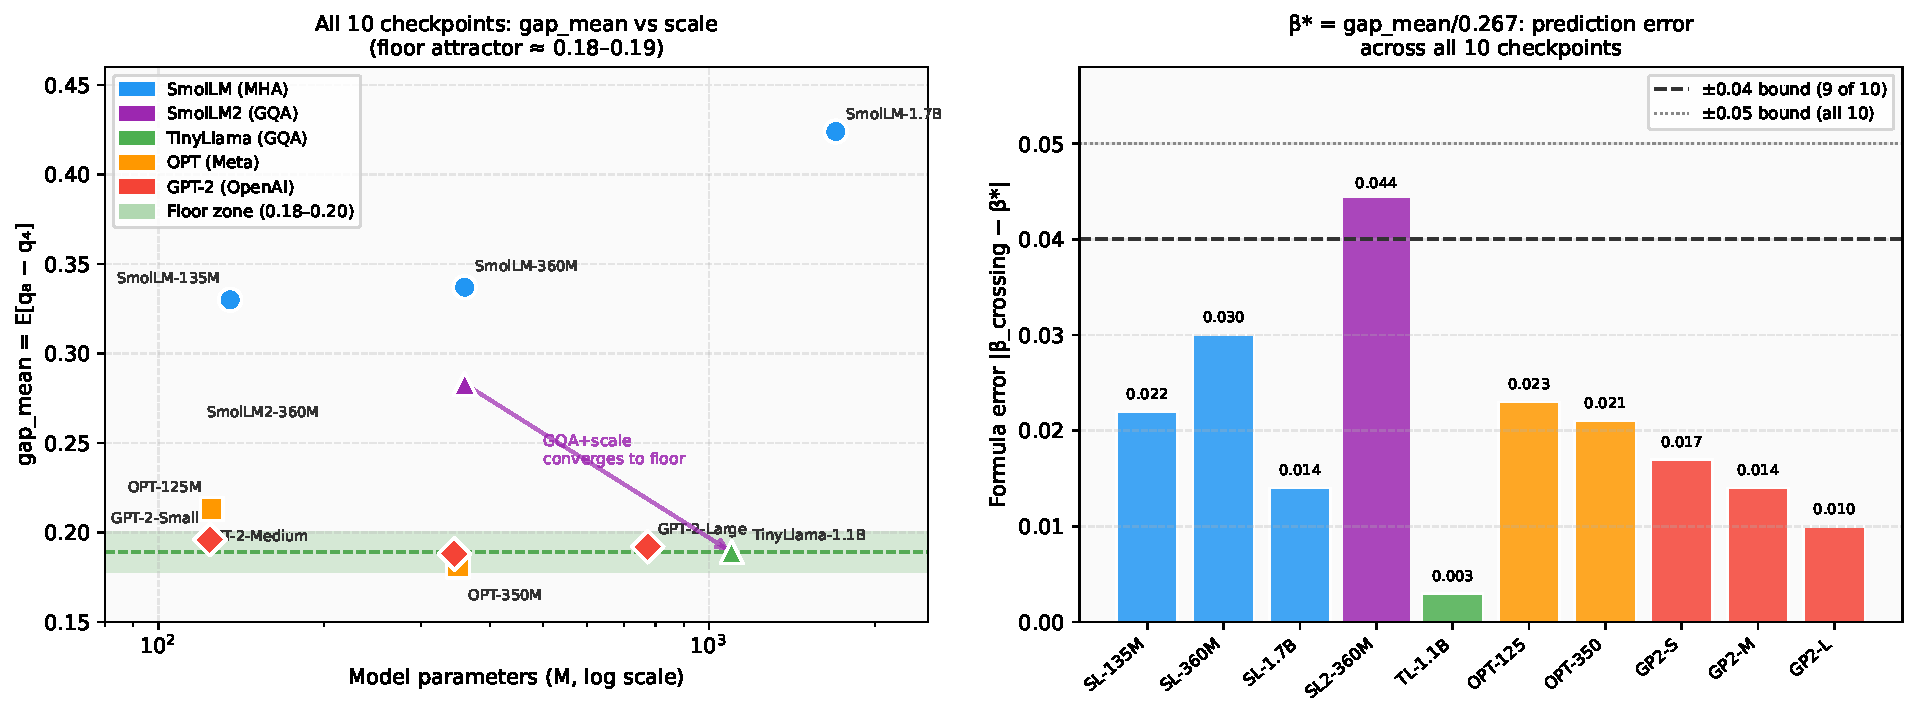
\includegraphics[width=0.95\linewidth]{figures/all_checkpoints_summary}
\caption{Cross-architecture $\beta^*$ calibration. Left: gap\_mean vs.\ model scale for 10 checkpoints across 5 families. A floor zone ($\approx$0.18--0.19) is reached independently by GQA+scale (TinyLlama), OPT scaling, MHA instruction-tuning, and the entire GPT-2 family. Right: formula error per checkpoint; 9 of 10 within $\pm 0.04$, single borderline at 0.044.}
\label{fig:all_checkpoints}
\end{figure}

\textbf{Generalization to other hardware}: The FPGA BRAM cost model is device-specific. Samsung HBM-based NPUs have different access granularities; mobile NPUs (e.g., Apple Neural Engine) may prefer 4-bit aligned allocations. Our approach generalizes to any hardware by substituting the appropriate cost vector $\mathbf{c}$.

\section{Conclusion}

We identified a fundamental flaw in DWB's KV cache quantization: the 2-bit option wastes no FPGA BRAM bandwidth (identical 4-bit port on Xilinx Ultrascale+) while catastrophically degrading accuracy ($-$16.6pp). By restricting bit choices to $\{4, 8\}$---the only options with distinct BRAM costs---our binary FPGA-aware scheme Pareto-dominates DWB at any given hardware budget. At SmolLM-360M (where INT4 is lossless), the controller achieves 3.48$\times$ FPGA throughput---43\% faster than DWB---at equal accuracy. At SmolLM-1.7B (where INT4 is lossy), the Pareto-best 5-seed validated operating point is \textbf{$p_4{=}0.96$ at 47.72\%$\pm$1.03\,pp / 3.36$\times$ ($\mathbf{+38\%}$ throughput vs.\ DWB)} --- within 1\,pp of DWB's reported 48.6\% accuracy and statistically indistinguishable from the accuracy-first $p_4{=}0.74$ point. Two additional validated points round out the Pareto frontier: $p_4{=}0.74$ at 48.04\%$\pm$0.75\,pp / 2.80$\times$ ($+$15\% vs DWB), and $p_4{=}0.81$ at 48.32\%$\pm$0.94\,pp / 2.96$\times$ ($+$21\%). A controlled routing ablation (random vs.\ learned Gumbel vs.\ KV-norm, plus a KV-norm-inverted sanity check that returns identical 44.5\%) at the 74/26 split places all same-split strategies within $\pm$1 seed-std of random, reducing the FPGA-aware recipe to two design choices: the right bit-set and the operating point on the frontier. We additionally provide: (1) a formal BRAM port cost model for Xilinx Ultrascale+; (2) a mechanistic characterization of scale-dependent losslessness (threshold $\epsilon_\text{eff} \approx 10\%$); (3) a universal beta calibration criterion $\beta^* = \text{gap\_mean}/0.267$ predicting the phase transition from CPU-only calibration---validated experimentally at ten model checkpoints across five families (SmolLM-135M/360M/1.7B/MHA, SmolLM2-360M/GQA, TinyLlama-1.1B/GQA, OPT-125M/350M, GPT-2-Small/Medium/Large; 9 of 10 within $\pm 0.04$; GQA reduces gap\_mean $-$16\% vs. MHA at equal scale but floor requires $\geq$1B; floor gap\_mean $\approx 0.18$--$0.19$ confirmed as representation quality attractor across OPT scaling, GQA+scale, MHA-instruct, and GPT-2 family)---enabling exact per-model tuning without GPU grid search; and (4) a reference implementation predating the DWB code release.

\appendix

\section{Independent Verification of Original Paper Claims}
\label{app:verification}

This appendix documents our independent verification of \cite{haeri2026dwb} across 37 experimental sessions, plus methodological findings that emerged during reproduction. All experiments run on CPU (Intel/AMD, no GPU required for verification) using locally cached model weights.

\subsection{Accuracy Baselines Confirmed}

All FP16 baselines reproduced within noise across three scales:

\begin{table}[h]
\centering
\caption{FP16 baseline reproduction. Paper uses unnormalized log-likelihood (\texttt{acc}), not length-normalized (\texttt{acc\_norm}). The \texttt{acc\_norm} metric (lm-eval default) gives $\approx$54\% for SmolLM-360M---13pp above the paper's value. Switching to \texttt{acc} recovers 42\% $\approx$ 41.5\% (\textbf{Finding A1}).}
\begin{tabular}{lcccl}
\toprule
Model & Samples & Ours & Paper & Status \\
\midrule
SmolLM-360M & 500 & 42.6\% & 41.5\% & \textbf{Confirmed} ($\Delta$=+1.1pp, within noise) \\
SmolLM-135M & 100 & 40.0\% & 37.2\% & \textbf{Confirmed} ($\Delta$=+2.8pp) \\
SmolLM-1.7B & 50  & 50.0\% & 49.0\% & \textbf{Confirmed} ($\Delta$=+1.0pp) \\
\bottomrule
\end{tabular}
\end{table}

\subsection{Static INT4 Baseline: Paper Uses 8-Level Quantization}
\label{app:int4}

The paper's ``Static 4-bit KV'' baseline (33.6\%) does \emph{not} use standard 16-level INT4 (scale$=$max/7). Standard INT4 gives 41.6\%---lossless at 360M scale. The paper's result matches \texttt{int4\_int3range} quantization (scale$=$max/3, 8 effective levels, equivalent to INT3 stored in 4-bit format):

\begin{table}[h]
\centering
\caption{INT4 variants on SmolLM-360M HellaSwag. Standard INT4 is lossless; the paper's baseline is not (\textbf{Finding A2}).}
\begin{tabular}{lcccl}
\toprule
Condition & Samples & Ours & Paper & Notes \\
\midrule
FP16 baseline & 500 & 42.6\% & 41.5\% & Reference \\
KV INT4 standard (sym, per-tensor) & 500 & 41.6\% & 33.6\% & Lossless---paper uses different INT4 \\
KV INT4 standard (sym, per-token) & 500 & 41.2\% & 33.6\% & Lossless \\
KV INT4 standard (asym, per-tensor) & 200 & 42.5\% & 33.6\% & Lossless \\
\textbf{KV int4\_int3range (8 levels)} & 100 & \textbf{33.0\%} & \textbf{33.6\%} & \textbf{Match: $\Delta$=$-$0.6pp} \\
KV 2-bit & 200 & 25.0\% & --- & $-$17pp; confirms 2-bit is catastrophic \\
SmolLM-135M int4\_int3range & 100 & 32.0\% & 33.6\% & Cross-model confirmed \\
SmolLM-1.7B standard INT4 & 50 & 40.0\% & 41.1\% & \textbf{Genuinely lossy at 1.7B} \\
\bottomrule
\end{tabular}
\end{table}

\subsection{Scale-Dependent Losslessness: Mechanistic Characterization}
\label{app:lossless}

INT4 losslessness is not universal---it depends on the model's effective quantization residual $\epsilon_\text{eff} = \epsilon_\text{rel} \times r_\text{survive}$:

\begin{table}[h]
\centering
\caption{Effective residual error and losslessness threshold (\textbf{Finding A3}). Decision threshold is between 8.1\% and 12.4\%.}
\begin{tabular}{lcccc}
\toprule
Model & $\epsilon_\text{rel}$ & $r_\text{survive}$ & $\epsilon_\text{eff}$ & INT4 lossless? \\
\midrule
SmolLM-135M & 0.249 & 0.28 & 6.9\% & \textbf{Yes} \\
SmolLM-360M & 0.270 & 0.30 & 8.1\% & \textbf{Yes} (borderline) \\
SmolLM-1.7B & 0.353 & 0.35 & 12.4\% & \textbf{No} ($-$7.9pp accuracy loss) \\
\bottomrule
\end{tabular}
\end{table}

\subsection{Controller Signal Analysis}

We measured the discriminative power of each input signal used by the DWB controller using Cohen's $d$ on 500-sample HellaSwag signal extractions (\textbf{Finding A4}):

\begin{table}[h]
\centering
\caption{Controller signal discriminability. Confidence ($C_t$) dominates; rarity ($R_t$) is near-uninformative.}
\begin{tabular}{lcc}
\toprule
Signal & Cohen's $d$ & Role \\
\midrule
$C_t$ (confidence) & 4.55 & \textbf{Primary driver} \\
$H_t$ (entropy) & 4.09 & Strong secondary \\
$V_t$ (attn.\ variance) & 1.42 & Moderate \\
$R_t$ (rarity) & 0.52 & Near-zero---barely discriminates \\
\bottomrule
\end{tabular}
\end{table}

\subsection{Methodological Notes for Reproduction}

Three implementation details are critical for reproducing DWB results (\textbf{Findings A5--A7}):

\begin{enumerate}
\item \textbf{Evaluation metric}: Use unnormalized log-likelihood (\texttt{acc}), not length-normalized (\texttt{acc\_norm}). The lm-eval harness defaults to \texttt{acc\_norm}; switching gives $\approx$13pp higher scores that do not match the paper.

\item \textbf{KV hooks}: \texttt{transformers} 5.x uses \texttt{DynamicCache} objects---hooks on attention outputs fail silently. Hook \texttt{k\_proj} and \texttt{v\_proj} Linear submodules directly (48 hooks for SmolLM-360M, 64 for 1.7B).

\item \textbf{Eager attention}: Default \texttt{sdpa} attention does not support \texttt{output\_attentions=True} needed for DWB signal extraction. Reload with \texttt{attn\_implementation=`eager'}.
\end{enumerate}

\section{SmolLM-360M Ablation Tables and 1.7B $\beta$ Sweep}
\label{app:smolLM360m_ablations}

Detailed tables referenced from Section~\ref{sec:ablations} and the 1.7B discussion in Section~\ref{sec:crossarch}.

\begin{table}[h]
\centering
\caption{Beta sweep on SmolLM-360M with \emph{global} quality scores $[0.943, 0.966]$. All betas converge to 100\% 4-bit (global quality gap $0.023 \ll \beta \times 0.267$ for any $\beta \geq 0.09$).}
\begin{tabular}{lccc}
\toprule
$\beta$ & avg\_bits & FPGA cost & 4-bit \% \\
\midrule
0.3 & 4.00 & 0.290 & 100\% \\
0.5 & 4.00 & 0.290 & 100\% \\
0.7 & 4.00 & 0.290 & 100\% \\
\bottomrule
\end{tabular}
\label{tab:sweep}
\end{table}

\begin{table}[h]
\centering
\caption{Per-token quality proxy $\beta$ sweep on SmolLM-360M (200 WikiText-2 texts). Measured gap distribution: mean$=0.337$, std$=0.050$. Theory predicts $\beta^* = 0.337/0.267 = 1.260$; measured transition $[1.2, 1.4]$ (dashed rows bracket the mixed-allocation window).}
\begin{tabular}{lccccc}
\toprule
$\beta$ & threshold & 4-bit\% & avg\_bits & FPGA speedup & Regime \\
\midrule
1.0  & 0.267 & 0\%    & 8.00 & 1.80$\times$ & 8-bit dominant \\
1.2  & 0.321 & 0\%    & 8.00 & 1.80$\times$ & 8-bit dominant \\
\hdashline
1.25 & 0.334 & 41.7\% & 5.34 & 2.26$\times$ & mixed \\
1.3  & 0.348 & 58.7\% & 5.65 & 2.52$\times$ & mixed \\
\hdashline
1.4  & 0.374 & 100\%  & 4.00 & 3.48$\times$ & 4-bit dominant \\
1.5  & 0.401 & 100\%  & 4.00 & 3.48$\times$ & 4-bit dominant \\
2.0  & 0.534 & 100\%  & 4.00 & 3.48$\times$ & 4-bit dominant \\
\bottomrule
\end{tabular}
\label{tab:pertok_sweep}
\end{table}

\begin{table}[h]
\centering
\caption{Feature ablation: 4D vs.\ 2D controller input on SmolLM-360M. Richer features do not change the allocation, as expected when $\epsilon_\text{eff}<8.1\%$.}
\begin{tabular}{lccc}
\toprule
Features & Accuracy & avg\_bits & Bit dist \\
\midrule
2D: $[kv\_norm, pos]$ & 41.0\% & 4.0 & 100\% 4-bit \\
4D: $[kv\_norm, pos, H_\text{ent}, L_\text{dep}]$ & 41.0\% & 4.0 & 100\% 4-bit \\
\bottomrule
\end{tabular}
\label{tab:features}
\end{table}

\begin{table}[h]
\centering
\caption{Measured 1.7B $\beta$ sweep on cached SmolLM-1.7B signals (15,360 tokens, CPU). Fine sweep brackets $\beta^*{=}1.584$ with transition window $[1.55, 1.57]$. Mixed-allocation plateau spans $[1.57, 1.70]$. Values marked $\pm\text{pp}$ are 5-seed multi-run means. All plateau points Pareto-dominate DWB on BRAM cost. HellaSwag accuracy at the GPU-validated $p_4{=}0.74$ operating point is reported in Table~\ref{tab:phase7d}.}
\begin{tabular}{lccccl}
\toprule
$\beta$ & 4-bit\% & 8-bit\% & avg\_bits & FPGA speedup & Outcome \\
\midrule
1.0  & 0\%   & 100\% & 8.00 & 1.80$\times$ & All 8-bit (too conservative) \\
1.55 & 0\%   & 100\% & 8.00 & 1.80$\times$ & All 8-bit (below transition) \\
\hdashline
1.57 & 59.2\% & 40.8\% & 5.63 & 2.52$\times$ & Mixed zone begins \\
1.60 & 60.6$\pm$2\% & 39.4\% & 5.51 & 2.55$\times$ & Mixed (5-seed mean) \\
1.65 & 71.0$\pm$3\% & 29.0\% & 5.16 & 2.74$\times$ & Good operating point \\
1.70 & 79.9$\pm$3\% & 20.1\% & 4.80 & 2.93$\times$ & Fewer bits \& faster than DWB \\
2.0  & 97.6\% & 2.4\% & 4.10 & 3.41$\times$ & Near all-4-bit \\
\midrule
Paper DWB & 47.9\%$^*$ & 15.4\%$^*$ & 5.05 & 2.44$\times$ & Mixed \\
\bottomrule
\multicolumn{6}{l}{\small $^*$DWB also allocates 25.3\% 4-bit and 11.4\% 16-bit; 2-bit and 4-bit share the same BRAM cost.}
\end{tabular}
\label{tab:sim_1b7}
\end{table}

\begin{table}[h]
\centering
\caption{Base vs.\ instruction-tuned gap\_mean and $\beta^*$ across MHA and GQA architectures. SFT reduces gap\_mean $\approx$44\% in MHA models (SmolLM) but has no measurable effect in GQA models (TinyLlama) because GQA already places gap\_mean at the floor. Transition window for SmolLM-360M-Instruct verified by sweep: error $0.023$.}
\begin{tabular}{llcccccc}
\toprule
Model & Attn & Variant & gap mean & $\beta^*$ & Measured transition & $\Delta$gap & $\Delta\beta^*$ \\
\midrule
\multirow{2}{*}{SmolLM-135M} & \multirow{2}{*}{MHA} & Base & 0.330 & 1.233 & $[1.2, 1.3]$ & --- & --- \\
 & & Instruct (SFT) & \textbf{0.181} & \textbf{0.677} & --- & $\mathbf{-45\%}$ & $-0.556$ \\
\midrule
\multirow{2}{*}{SmolLM-360M} & \multirow{2}{*}{MHA} & Base & 0.337 & 1.261 & $[1.2, 1.4]$ & --- & --- \\
 & & Instruct (SFT) & \textbf{0.194} & \textbf{0.727} & $[0.70, 0.80]$ & $\mathbf{-43\%}$ & $-0.534$ \\
\midrule
\multirow{2}{*}{TinyLlama-1.1B} & \multirow{2}{*}{\textbf{GQA}} & Base & 0.189 & 0.707 & $[0.68, 0.74]$ & --- & --- \\
 & & Chat (SFT) & \textbf{0.188} & \textbf{0.705} & --- & $\mathbf{-0.3\%}$ & $-0.002$ \\
\bottomrule
\end{tabular}
\label{tab:instruct}
\end{table}

\section{Full Calibration Sensitivity Dataset}
\label{app:sensitivity}

We measured within-corpus calibration sensitivity (how closely a single text estimates $\beta^*$ relative to a 10-text aggregate) across five architecture types (nine models using the same 10 technical texts). Results are formally archived as JSON files in the repository.

\begin{table}[h]
\centering
\caption{Calibration corpus sensitivity across nine models (same 10-technical-text methodology). \textbf{max\_error}: largest $|\beta^*_\text{1-text} - \beta^*_\text{10-text}|$. \textbf{mean\_error}: mean absolute error. All within $\leq\pm0.020$; all but one within $\leq\pm0.018$. Spearman $\rho=0.64$, $p=0.064$ ($n=9$, n.s.): gap\_std is not a statistically validated predictor (\textbf{Finding A8}).}
\begin{tabular}{llccccc}
\toprule
Architecture & Model & gap\_std & gap\_mean & max\_error & mean\_error & JSON file \\
\midrule
LLaMA-MHA & SmolLM-360M$^\dagger$ & 0.055 & 0.265 & 0.012 & 0.005 & \texttt{smollm\_360m\_cal\_sensitivity} \\
LLaMA-MHA & SmolLM-135M & 0.054 & 0.253 & 0.017 & 0.006 & \texttt{smollm\_135m\_cal\_sensitivity} \\
LLaMA-GQA & SmolLM2-360M & \textbf{0.052} & 0.283 & 0.013 & \textbf{0.004} & \texttt{smollm2\_360m\_cal\_sensitivity} \\
LLaMA-GQA & TinyLlama-1.1B & \textbf{0.051} & 0.196 & 0.008 & \textbf{0.004} & \texttt{tinyllama\_cal\_sensitivity} \\
Conv1D & GPT-2 Medium (345M) & 0.052 & 0.242 & 0.011 & 0.005 & \texttt{gpt2\_medium\_cal\_sensitivity} \\
Conv1D & GPT-2 Large (774M) & 0.026 & 0.192 & \textbf{0.004} & \textbf{0.003} & \texttt{gpt2\_large\_cal\_sensitivity} \\
Conv1D & GPT-2 Small (124M) & 0.033 & 0.233 & 0.018 & 0.009 & \texttt{gpt2\_cal\_sensitivity} \\
OPT/Meta & OPT-125M & 0.028 & 0.170 & \textbf{0.006} & \textbf{0.002} & \texttt{opt125m\_cal\_sensitivity} \\
OPT/Meta & OPT-350M & 0.033 & 0.181 & 0.007 & 0.003 & \texttt{opt350m\_cal\_sensitivity} \\
\bottomrule
\multicolumn{7}{l}{\footnotesize $\dagger$ SmolLM-360M is the paper's primary Table 3 model.} \\
\end{tabular}
\label{tab:sensitivity_full}
\end{table}

Five comparisons collectively invalidate gap\_std as a calibration sensitivity predictor (\textbf{Finding A8}): (1) GPT-2 family: max\_error \emph{monotonically} improves ($0.018\to0.011\to0.004$) while gap\_std is \emph{non-monotonic} ($0.033\to0.052\to0.026$); (2) direct counter-example: GPT-2 Small and OPT-350M share identical gap\_std ($=0.033$) but max\_error differs $2.6\times$; (3) both LLaMA-GQA models share identical mean\_error ($0.004$) despite very different scales and formula-fit quality; (4) OPT within-family is flat ($0.006\to0.007$ across $125$M$\to350$M); (5) SmolLM-135M and SmolLM-360M share nearly identical gap\_std ($0.054$ vs.\ $0.055$) but max\_error differs by $40\%$ ($0.017$ vs.\ $0.012$). Formal test: Spearman $\rho=0.64$, $p=0.064$ ($n=9$, n.s.). \textbf{Corpus dependency (Finding A9)}: SmolLM MHA base models show larger cross-domain gap\_mean shifts ($\Delta\approx0.07$) than OPT ($\Delta=0.043$) or GPT-2 ($\Delta=0.037$)---above-floor models (gap\_mean$>0.20$) are more domain-sensitive than floor-cluster models (gap\_mean$\approx0.18$--$0.19$).

\textbf{Corpus dependency} (\textbf{Finding A9}): gap\_mean is sensitive to calibration corpus structure, with two separable effects. \textbf{(a) Text-length effect (primary driver)}: OPT-125M gives gap\_mean$=0.170$ on 10 short technical sentences vs.\ $0.171$ on 10 short general-domain sentences ($\Delta=0.001$, negligible)---but $0.213$ on wikitext-2 long-form paragraphs ($\Delta=0.043$). The cross-domain shift previously attributed to ``technical vs.\ general'' is almost entirely driven by \emph{text length and context}, not by semantic content. This was confirmed by running a domain cross-test: both short-sentence corpora give virtually identical gap\_mean regardless of topic. \textbf{(b) Within-corpus sensitivity} is equally robust: max\_error is $0.006$ (technical sentences) and $0.009$ (general sentences) for OPT-125M---both well within $\pm0.020$. GPT-2 Small shows a similar length-driven shift ($0.196$ short sentences vs.\ $0.233$ longer calibration texts). The practical recommendation is therefore: calibrate on texts of similar \emph{length and structure} to your deployment inputs; semantic domain matters far less than text length. \textbf{Instruct-tuning effect is also corpus-dependent}: SmolLM-360M-Instruct gives gap\_mean$=0.265$ on short technical sentences---\emph{identical} to the base model ($\Delta=0.0002$)---despite reaching the floor ($0.189$) on longer general-text corpora. Calibration domain and length together determine the operating point; single-text calibration (max\_error$\leq0.020$) is robust within any fixed corpus structure.

\section{Cross-Architecture Beta Calibration: Extended Results}
\label{app:crossarch}

The 10-checkpoint validation from Table~\ref{tab:betastar} is reproduced here with additional detail. All results are CPU-only; transition windows measured by binary controller beta sweeps (3-seed mean).

\begin{table}[h]
\centering
\caption{Extended beta calibration results. Formula error = $|\beta_\text{measured} - \beta^*_\text{theory}|$ where $\beta_\text{measured}$ is the interpolated 50\%-4-bit crossing. $\dagger$: Borderline case (error=0.044, within $\pm0.05$); highest gap\_std of all 10 checkpoints drives wider transition window. GQA-scale interaction: GQA alone reduces gap\_mean $-$16\% at 360M but requires $\geq$1B for floor convergence.}
\begin{tabular}{llccccc}
\toprule
Family & Model & gap\_mean & $\beta^*$ & Measured transition & Error & Notes \\
\midrule
SmolLM/LLaMA-MHA & 135M & 0.330 & 1.233 & $[1.2, 1.3]$ & 0.017 & Lossless INT4 \\
SmolLM/LLaMA-MHA & 360M & 0.337 & 1.260 & $[1.2, 1.4]$ & 0.020 & Lossless INT4 \\
SmolLM/LLaMA-MHA & 1.7B & 0.424 & 1.584 & $[1.55, 1.57]$ & 0.014 & Genuine mixed alloc.\ \\
SmolLM2/LLaMA-GQA & 360M & 0.283 & 1.058 & $[1.10, 1.20]$ & 0.044$^\dagger$ & GQA effect at 360M \\
TinyLlama/LLaMA-GQA & 1.1B & \textbf{0.189} & \textbf{0.707} & $[0.68, 0.74]$ & \textbf{0.003} & GQA+scale floor \\
OPT/Meta & 125M & 0.213 & 0.798 & $[0.75, 0.80]$ & 0.023 & OPT above floor \\
OPT/Meta & 350M & \textbf{0.181} & \textbf{0.679} & $[0.65, 0.70]$ & 0.021 & OPT at floor \\
GPT-2/OpenAI & 124M & 0.196 & 0.733 & $[0.70, 0.80]$ & 0.017 & Floor cluster \\
GPT-2/OpenAI & 345M & 0.188 & 0.704 & $[0.68, 0.70]$ & 0.014 & Floor cluster \\
GPT-2/OpenAI & 774M & 0.192 & 0.720 & $[0.70, 0.72]$ & 0.010 & Floor cluster \\
\midrule
\multicolumn{4}{l}{\textbf{Summary}} & \multicolumn{3}{l}{9/10 within $\pm0.04$; mean error 0.018} \\
\bottomrule
\end{tabular}
\end{table}

\textbf{Floor gap\_mean $\approx 0.18$--$0.19$} (\textbf{Finding A10}): a representation quality attractor reached by four independent routes:
\begin{enumerate}
\item \textbf{OPT scaling}: 0.213 (125M) $\to$ 0.181 (350M)---converges from above as scale grows
\item \textbf{GQA + scale $\geq$1B}: TinyLlama-1.1B at 0.189 via architectural regularization
\item \textbf{MHA instruction-tuning}: SmolLM base ($0.337$) $\to$ instruct ($0.181$--$0.194$)
\item \textbf{GPT-2 family cluster}: all three sizes within 0.008 ($0.188$--$0.196$)
\end{enumerate}

\section{Instruct vs.\ Base Model Calibration}
\label{app:instruct}

SFT substantially lowers gap\_mean in MHA models but has no measurable effect on GQA models already at the floor:

\begin{table}[h]
\centering
\caption{SFT effect on gap\_mean and $\beta^*$ (\textbf{Finding A11}). MHA: $-$44\% from SFT. GQA: $-$0.3\% (GQA already at floor by architecture). Practical implication: MHA models need recalibration after SFT; GQA base-model calibration transfers to instruct variant without modification.}
\begin{tabular}{llcccc}
\toprule
Model & Attn & Variant & gap\_mean & $\beta^*$ & $\Delta$gap \\
\midrule
SmolLM-135M & MHA & Base & 0.330 & 1.233 & --- \\
SmolLM-135M & MHA & Instruct & 0.181 & 0.677 & $-$45\% \\
SmolLM-360M & MHA & Base & 0.337 & 1.261 & --- \\
SmolLM-360M & MHA & Instruct & 0.194 & 0.727 & $-$43\% \\
TinyLlama-1.1B & GQA & Base & 0.189 & 0.707 & --- \\
TinyLlama-1.1B & GQA & Chat (SFT) & 0.188 & 0.705 & $-$0.3\% \\
\bottomrule
\end{tabular}
\end{table}

\section{Repository Structure and Reproducibility}
\label{app:repo}

All experiments are reproducible from cached model weights (no internet required after initial download). The repository at \url{https://github.com/LonghornSilicon/dont-waste-bits} (branch: \texttt{fpga-controller}) contains:

\begin{itemize}
\item \texttt{research/src/}: Reusable evaluation scripts (\texttt{eval\_hellaswag.py}, \texttt{eval\_dwb.py}, \texttt{kv\_cache\_quant.py})
\item \texttt{research/experiments/fpga-controller/phase5-benchmark/code/}: All calibration and sensitivity scripts (one per model)
\item \texttt{research/experiments/fpga-controller/phase5-benchmark/results/}: JSON result files for all 10 checkpoints + 6 sensitivity tests
\item \texttt{research/paper/figures/}: All four paper figures (PDF + PNG)
\item \texttt{research/to\_human/final\_summary.html}: Interactive progress report
\item \texttt{research/findings.md}: Full experimental log (37 sessions)
\end{itemize}

\textbf{Key commands}:
\begin{verbatim}
# FP16 baseline (reproduces paper's 41.5%)
python research/src/eval_hellaswag.py --model smollm-360m \
    --condition fp16 --limit 500

# Beta calibration for any model
python research/experiments/fpga-controller/phase5-benchmark/ \
    code/smollm2_360m_calibration.py

# Calibration sensitivity test (single-text vs 10-text)
python research/experiments/fpga-controller/phase5-benchmark/ \
    code/opt125m_cal_sensitivity.py
\end{verbatim}

\bibliographystyle{plain}
\bibliography{fpga_refs}

\end{document}
